\documentclass[tikz,border=10pt]{standalone}
\usetikzlibrary{calc}

\begin{document}
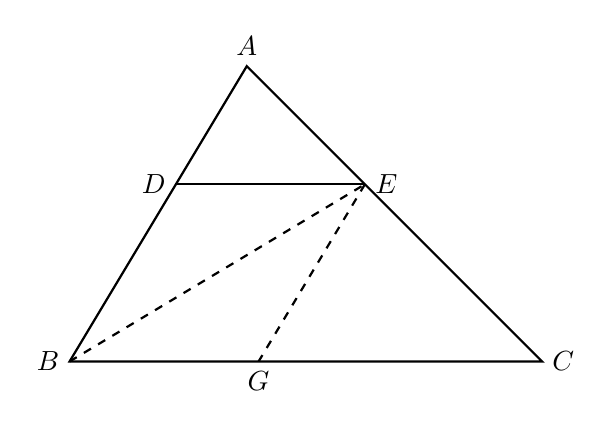
\begin{tikzpicture}[thick, scale=1.5]
    % 1. 定义顶点坐标
    \coordinate (B) at (0,0);
    \coordinate (C) at (4,0);
    \coordinate (A) at (1.5,2.5);
    
    % 定义D点在AB上的位置 (例如 0.6*A + 0.4*B)
    \coordinate (D) at ($(A)!0.4!(B)$);
    % 定义E点在AC上的位置 (即与D等比例，保证平行)
    \coordinate (E) at ($(A)!0.4!(C)$);
    % 定义G点在BC上的位置
    \coordinate (G) at (1.6,0);

    % 2. 绘制三角形轮廓和平行线
    \draw (A) -- (B) -- (C) -- cycle;
    \draw (D) -- (E);

    % 3. 绘制虚线辅助线
    \draw[dashed] (B) -- (E);
    \draw[dashed] (E) -- (G);

    % 4. 标注节点名称
    \node[above] at (A) {$A$};
    \node[left]  at (B) {$B$};
    \node[right] at (C) {$C$};
    \node[left]  at (D) {$D$};
    \node[right] at (E) {$E$};
    \node[below] at (G) {$G$};

\end{tikzpicture}
\end{document}